\documentclass[letterpaper,journal]{IEEEtran}
% Format follows the supplied HCDP.tex; redundant/conflicting packages removed.
\usepackage{amsmath,amssymb,amsthm}
\usepackage{algorithm,algorithmic}
\renewcommand{\algorithmicrequire}{\textbf{Input:}}
\renewcommand{\algorithmicensure}{\textbf{Output:}}
\usepackage{array,booktabs,tabularx,multirow,graphicx}
\usepackage{stfloats,url}
\usepackage[numbers,sort&compress]{natbib}
\usepackage[hidelinks]{hyperref}
\usepackage{tikz,pgfplots}
\usetikzlibrary{arrows.meta,positioning,fit}
\pgfplotsset{compat=1.18}
\newtheorem{proposition}{Proposition}
\newcommand{\etal}{\textit{et al.}}
\newcommand{\IP}{\mathrm{IP}}
\newcommand{\LP}{\mathrm{LP}}
\newcommand{\LB}{\mathrm{LB}}
\newcommand{\UB}{\mathrm{UB}}
\newcommand{\drafttitle}{Whole-Line Column Generation for Multi-Line Human--Robot Collaborative Selective Disassembly With Cumulative Fatigue}
\hyphenation{dis-as-sem-bly work-station re-man-u-fac-tur-ing}
\setlength{\emergencystretch}{1em}

\begin{document}
\title{\drafttitle}
\author{Author Names and Affiliations to Be Confirmed}
\markboth{Research Manuscript Draft, November 2026}{Whole-Line Column Generation for Selective Disassembly}
\maketitle
\begin{abstract}
Multi-line disassembly requires coordination of limited human and robot resources for profitable material recovery.
This work considers selective task execution, three operation modes, AND precedence relationships, and cumulative station fatigue.
A mixed-integer linear model maximizes net profit under cycle-time, recovery, and shared-resource constraints.
A whole-line column generation framework integrates feasible line plans, two-phase resource coordination, restricted integer recovery, and demand-driven resource-profile bounds.
Computational experiments establish integer optimality for six synthetic instances with 80 or 120 tasks in 19.36--182.69 seconds under a 600-second protocol, whereas direct compact-model optimization remains unproven on these instances; additional resource-constrained cases confirm the benefit, and a difficult two-line case identifies its boundary.
\end{abstract}
\begin{IEEEkeywords}
Human--robot collaboration, disassembly line balancing, column generation, cumulative fatigue, resource allocation.
\end{IEEEkeywords}
\section{Introduction}\label{sec:intro}
\IEEEPARstart{D}{isassembly} supports the recovery of reusable components and materials from end-of-life products. A disassembly line balancing problem (DLBP) assigns selected tasks to ordered workstations. Task selection affects recovery value. Workstation allocation affects time, resource demand, and operating cost. Guo \etal\ describe the modeling and optimization challenges in disassembly sequence planning \cite{Guo2021}.

Human--robot collaboration provides several task execution options. A human can perform a manual task, a robot can perform an automated task, and a joint mode can use both resources. Guo \etal\ study stochastic operation time with a multi-objective shuffled frog leaping method \cite{Guo2024a}. Guo \etal\ also examine partial destructive disassembly with human--robot hybrid operation \cite{Guo2024}. Chu and Chen examine selective operations in a two-sided cooperative line \cite{Chu2025}. Huang \etal\ consider uncertain operation and equipment activation in a U-shaped line \cite{Huang2025}. These studies motivate explicit execution-mode and resource decisions. Their layouts and objectives differ from the multi-line setting considered here.

Coordination becomes important when several lines draw resources from common pools. Local plans can satisfy every task and station requirement, yet their combined staffing demand can exceed the available resources. Guo \etal\ model multiproduct collaborative hybrid lines with resource sharing and solve them with a discrete aquila optimizer \cite{Guo2025}. Gu \etal\ address shared transportation in multi-factory remanufacturing \cite{Gu2025}. Zhou \etal\ consider worker fatigue in multi-factory process optimization \cite{Zhou2025}. These studies establish the relevance of resource coordination and human factors. The present work focuses on fixed human and robot deployment across disassembly lines. It uses a station-level fatigue limit over one representative cycle. Its computational contribution concerns line-plan decomposition and auditable integer bounds, rather than the general introduction of resource sharing.

A compact mixed-integer linear programming (MILP) formulation provides a direct optimization model. Its relaxation can mix fractional task assignments within stations. An alternative formulation represents an entire feasible line plan by one column. All line-specific constraints then remain inside the pricing domain. Only two resource capacities connect the lines. Dantzig and Wolfe establish the decomposition principle for block-structured models \cite{Dantzig1960}. L\"ubbecke and Desrosiers explain the role of pricing and dual bounds in column generation (CG) \cite{Lubbecke2005}. This theory motivates the present formulation; decomposition itself is an established method.

The computational question is whether line-level convexification reduces the cost of obtaining profitable, certifiable integer plans. A stronger relaxation alone does not answer this question. Each pricing problem remains an integer optimization problem. Large line blocks can make pricing expensive. Fractional master solutions can also leave an integer gap. A practical framework therefore needs both line pricing and a separate mechanism for integer solutions and bounds.

This work makes three contributions. First, it formulates a profit-maximizing multi-line DLBP with selective tasks, three execution modes, cumulative fatigue, and shared resource pools. Second, it develops a whole-line reformulation with an integer equivalence proof, two-phase CG, and demand-driven resource-profile coordination. Third, it evaluates the framework against direct compact-model optimization on frozen synthetic inputs. The evaluation reports valid bounds and proof states as well as execution time. It also identifies a failure regime with few, large pricing blocks.

Section~\ref{sec:model} defines the problem and compact model. Section~\ref{sec:method} presents the decomposition and integer coordination. Section~\ref{sec:experiments} reports the computational evidence. Section~\ref{sec:conclusion} states the conclusions and remaining questions.

\section{Problem Description and Mathematical Model}\label{sec:model}
\subsection{System Definition and Assumptions}
Each line has its own task set and an AND precedence graph. An executed successor requires every direct predecessor. Optional tasks can remain unexecuted. Required tasks must be executed. Each selected task receives one allowed mode and one station. Stations have ordered indices. A predecessor can occupy the same station as its successor. A topological order provides a feasible within-station sequence.

Modes H, R, and J denote human, robot, and joint execution. Mode J requires one human and one robot. Its duration enters station time once. Tasks within a station execute sequentially. Resource pools limit the total number of stations with human and robot deployment. This planning model does not describe resource movement between stations during operation.

Fatigue starts at zero in a representative cycle. Each human-involving task contributes a nonnegative additive load. The model contains no within-cycle recovery. It does not describe fatigue accumulation across successive cycles or an entire work shift. Robot-only modes have zero fatigue load. Candidate stations can have different costs. The formulation does not require consecutive station activation.

\begin{table}[!t]
\caption{Sets and Parameters}\label{tab:notation}\centering\small
\begin{tabularx}{\columnwidth}{@{}lX@{}}\toprule
Symbol&Definition\\\midrule
$\mathcal L$&Set of disassembly lines; index $l$.\\
$\mathcal I_l,\mathcal I_l^{\rm req}$&Tasks and required tasks of line $l$; index $i$.\\
$\mathcal S_l=\{1,\ldots,k_l\}$&Ordered candidate stations; index $s$.\\
$\mathcal M_{li}\subseteq\{H,R,J\}$&Allowed execution modes; index $m$.\\
$\mathcal E_l$&Direct AND precedence arcs $(i,j)$.\\
$n_l$&Number of tasks on line $l$.\\
$v_{li},w_{li}$&Recovery value and recovery weight of task $i$.\\
$c_{li}^{m},t_{li}^{m},\beta_{li}^{m}$&Execution cost, duration, and fatigue coefficient.\\
$c_{ls}^{0},c_{ls}^{H},c_{ls}^{R}$&Activation, human, and robot costs.\\
$t_l^c,\bar f_l,b_l$&Cycle time, fatigue threshold, and fatigue budget.\\
$q_l$&Minimum recovery weight of line $l$.\\
$h^{\max},r^{\max}$&Shared human and robot capacities.\\
\bottomrule\end{tabularx}
\end{table}

\subsection{Compact Formulation}
Table~\ref{tab:notation} defines the main notation. Binary $y_{li}$ selects task $i$. Binary $x_{lism}$ assigns task $i$ to station $s$ in mode $m$. Binary $u_{ls}$, $h_{ls}$, and $r_{ls}$ indicate station activation, human deployment, and robot deployment. Let $a_m^H$ and $a_m^R$ be resource indicators. Their pairs are $(1,0)$, $(0,1)$, and $(1,1)$ for H, R, and J.

The objective maximizes net profit:
\begin{align}
\max\ z={}&\sum_{l,i}v_{li}y_{li}-\sum_{l,i,s,m}c_{li}^{m}x_{lism}\nonumber\\
&-\sum_{l,s}\left(c_{ls}^{0}u_{ls}+c_{ls}^{H}h_{ls}+c_{ls}^{R}r_{ls}\right).\label{eq:obj}
\end{align}
Every sum over $m$ uses the allowed set $\mathcal M_{li}$. The assignment and required-task constraints are
\begin{align}
\sum_{s\in\mathcal S_l}\sum_{m\in\mathcal M_{li}}x_{lism}&=y_{li}&&\forall l,i,\label{eq:assign}\\
y_{li}&=1&&\forall l,\ i\in\mathcal I_l^{\rm req}.\label{eq:required}
\end{align}
AND precedence uses cumulative prefixes for all $l$, $(i,j)\in\mathcal E_l$, and $k\in\mathcal S_l$:
\begin{equation}
\sum_{s=1}^{k}\sum_{m\in\mathcal M_{lj}}x_{ljsm}
\leq\sum_{s=1}^{k}\sum_{m\in\mathcal M_{li}}x_{lism}.\label{eq:prec}
\end{equation}
The final prefix enforces predecessor selection. Earlier prefixes enforce station order. Each station satisfies
\begin{align}
\sum_{i,m}t_{li}^{m}x_{lism}&\leq t_l^c u_{ls},\label{eq:cycle}\\
u_{ls}\leq\sum_{i,m}x_{lism}&\leq n_lu_{ls},\label{eq:active}\\
h_{ls}\leq\sum_{i,m}a_m^Hx_{lism}&\leq n_lh_{ls},\label{eq:hlogic}\\
r_{ls}\leq\sum_{i,m}a_m^Rx_{lism}&\leq n_lr_{ls},\label{eq:rlogic}\\
\sum_{i,m}d_{li}^{m}x_{lism}&\leq b_lh_{ls}.\label{eq:fatigue}
\end{align}
These constraints apply to all $l,s$. The fatigue load is $d_{li}^{m}=\beta_{li}^{m}t_{li}^{m}$. The budget is $b_l=-\ln(1-\bar f_l)$. Thus the fatigue level $1-\exp(-\sum_{i,m}d_{li}^{m}x_{lism})$ does not exceed $\bar f_l$. The deployment constraints make $h_{ls}=0$ exactly when no selected mode needs a human. Equivalent logic holds for robots and station activation. An empty station has zero deployment and zero activation cost.

Shared resources and line recovery satisfy
\begin{align}
\sum_{l,s}h_{ls}&\leq h^{\max},&\sum_{l,s}r_{ls}&\leq r^{\max},\label{eq:shared}\\
\sum_{i\in\mathcal I_l}w_{li}y_{li}&\geq q_l&&\forall l.\label{eq:recovery}
\end{align}
All decision variables are binary. Equations~\eqref{eq:assign}--\eqref{eq:recovery} retain the task, precedence, mode, cycle-time, fatigue, and recovery definitions of the implemented compact model. There are no precedence arcs between different lines.

\section{Proposed Algorithm}\label{sec:method}
\subsection{Whole-Line Plans}
Let $\mathcal X_l$ contain all binary solutions of line $l$ that satisfy \eqref{eq:assign}--\eqref{eq:fatigue} and \eqref{eq:recovery}. The shared limits in \eqref{eq:sharedh} and \eqref{eq:sharedr} remain outside this set. A pricing model can use the redundant bounds $\sum_s h_{ls}\leq k_l$ and $\sum_s r_{ls}\leq k_l$. These bounds do not allocate global resources to a line.

A column $p\in\mathcal P_l$ represents one complete plan in $\mathcal X_l$. It records the selected tasks, their stations and modes, and the associated station configurations. Define
\begin{align}
h_{lp}&=\sum_s h_{ls}^p,&r_{lp}&=\sum_s r_{ls}^p,\label{eq:features}\\
c_{lp}&=\sum_i v_{li}y_{li}^p-\sum_{i,s,m}c_{li}^{m}x_{lism}^p\nonumber\\
&\quad-\sum_s(c_{ls}^{0}u_{ls}^p+c_{ls}^{H}h_{ls}^p+c_{ls}^{R}r_{ls}^p).\label{eq:colprofit}
\end{align}
An empty station is allowed within a plan. A completely empty line plan exists only if the required-task and recovery conditions allow it. Columns with the same selected task set can still differ in station assignment or mode. Deduplication therefore uses the complete assignment pattern.

\begin{figure*}[!t]\centering
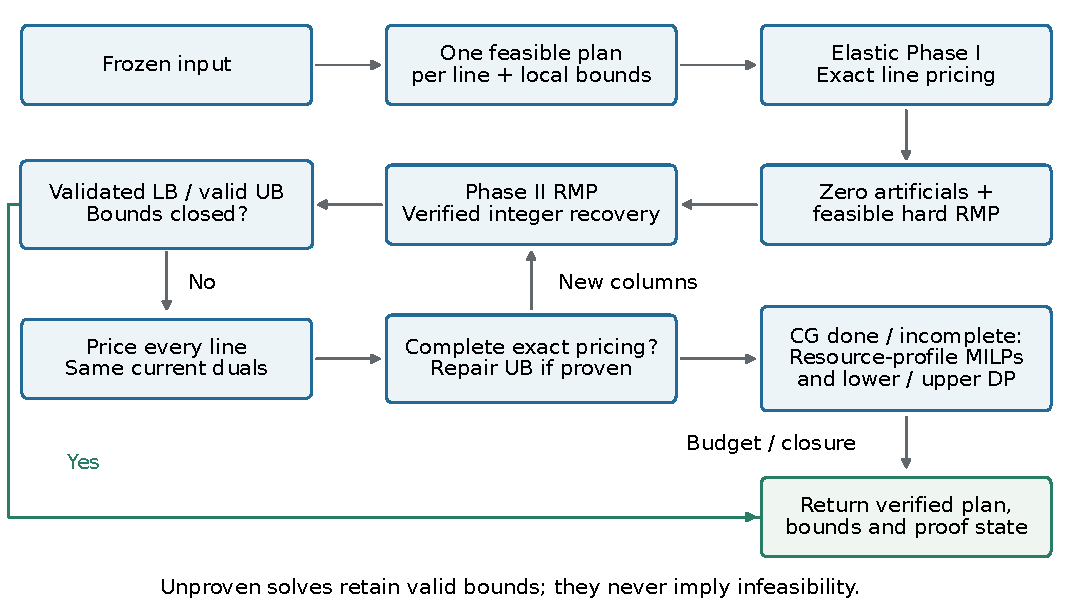
\includegraphics[width=\textwidth]{img/algorithm_flowchart.pdf}
\caption{Proposed framework. CG coordinates complete line plans; verified integer recovery and resource-profile bounds provide separate integer proof paths. Only complete exact pricing repairs the CG dual bound. A budget stop returns the actual proof state and remaining gap.}\label{fig:flow}
\end{figure*}
Fig.~\ref{fig:flow} shows the solution workflow. A station-level column can be locally feasible but difficult to combine across stations. A whole-line column already satisfies task uniqueness, required-task selection, all precedence prefixes, and line recovery. Integer combination then requires coordination of the two resource totals. The two-phase CG loop supplies LP coordination, while restricted integer recovery and profile queries address the remaining integer gap.

\subsection{Master Problem and Formulation Strength}
Binary $\lambda_{lp}$ selects one plan for line $l$. The complete master problem is
\begin{align}
\max\quad&\sum_l\sum_{p\in\mathcal P_l}c_{lp}\lambda_{lp},\label{eq:master}\\
\text{s.t.}\quad&\sum_{p\in\mathcal P_l}\lambda_{lp}=1&&\forall l,\label{eq:convex}\\
&\sum_{l,p}h_{lp}\lambda_{lp}\leq h^{\max},\label{eq:masterh}\\
&\sum_{l,p}r_{lp}\lambda_{lp}\leq r^{\max},\label{eq:masterr}\\
&\lambda_{lp}\in\{0,1\}.\label{eq:masterbinary}
\end{align}
Column profit already includes all station and resource costs.

\begin{proposition}\label{prop:equiv}
The complete integer master and the compact MILP have the same feasible objective values.
\end{proposition}
\begin{proof}
Extract the binary variables of each line from a feasible compact solution. They form a member of $\mathcal X_l$ and hence a column. Selecting these columns preserves the resource totals and every objective term. Conversely, select one column per line from a feasible integer master solution. Copy its task, station, and mode variables to the compact model. Local feasibility follows from $\mathcal X_l$. Shared feasibility follows from \eqref{eq:masterh} and \eqref{eq:masterr}. The two-way configuration logic fixes activation and deployment, including empty stations. The reconstructed profit is unchanged.
\end{proof}

The complete linear programming (LP) relaxation replaces \eqref{eq:masterbinary} by $\lambda_{lp}\geq0$. Let $z_{\rm line}^{\LP}$, $z_{\rm station}^{\LP}$, and $z_{\rm compact}^{\LP}$ denote the complete line, complete station, and compact LP bounds. Then
\begin{equation}
z^{\IP}\leq z_{\rm line}^{\LP}\leq z_{\rm station}^{\LP}\leq z_{\rm compact}^{\LP}.\label{eq:hierarchy}
\end{equation}
Every line-plan mixture induces station-plan mixtures with identical weights and objective. Station-plan mixtures in turn induce feasible compact fractional assignments. This establishes the inclusions in \eqref{eq:hierarchy}. The supplementary file gives the detailed mapping. These comparisons concern complete column sets, not arbitrary restricted pools.

\subsection{Restricted Master and Exact Pricing}
CG maintains a finite pool $\overline{\mathcal P}_l\subseteq\mathcal P_l$. Its restricted master problem (RMP) uses the LP version of \eqref{eq:master}--\eqref{eq:masterr} over this pool. The dual variables are $\sigma_l\in\mathbb R$ for \eqref{eq:convex} and $\pi_H,\pi_R\geq0$ for the resource rows. The complete dual is
\begin{align}
\min\quad&D=\sum_l\sigma_l+h^{\max}\pi_H+r^{\max}\pi_R,\label{eq:dual}\\
\text{s.t.}\quad&\sigma_l+\pi_Hh_{lp}+\pi_Rr_{lp}\geq c_{lp}&&\forall l,p.
\end{align}
The reduced cost of a column is
\begin{equation}
\bar c_{lp}=c_{lp}-\pi_Hh_{lp}-\pi_Rr_{lp}-\sigma_l.\label{eq:rc}
\end{equation}
Pricing solves one MILP per line:
\begin{equation}
\rho_l=\max_{p\in\mathcal P_l}\{c_{lp}-\pi_Hh_{lp}-\pi_Rr_{lp}-\sigma_l\}.\label{eq:pp}
\end{equation}
The objective increases the effective deployment costs by $\pi_H$ and $\pi_R$. All line constraints remain unchanged. Task coverage and precedence do not have separate master duals in this formulation. They belong to the pricing domain.

A new legal column enters the pool if its independently recomputed reduced cost exceeds $\varepsilon_{rc}$. All lines use the same RMP dual solution in a round. The implementation reuses one native CPLEX model per line. It updates every objective coefficient and submits the previous full integer solution as a warm start. Separate line sessions prevent state contamination.

\subsection{Initialization and Phase I}
A short economic MILP first seeks a feasible plan on each line. A constant-objective solve provides a fallback. A proven empty local domain implies global infeasibility. A time limit without a plan does not establish emptiness.

Local plans can conflict in their combined resource demands. Phase I keeps each convexity equation hard and adds nonnegative elastic variables:
\begin{align}
\max\quad&-a_H-a_R,\label{eq:p1}\\
\text{s.t.}\quad&\sum_p\lambda_{lp}=1&&\forall l,\nonumber\\
&\sum_{l,p}h_{lp}\lambda_{lp}-a_H\leq h^{\max},\nonumber\\
&\sum_{l,p}r_{lp}\lambda_{lp}-a_R\leq r^{\max},\nonumber\\
&\lambda_{lp},a_H,a_R\geq0.\nonumber
\end{align}
One local plan per line makes this elastic RMP feasible. Real columns have zero objective coefficients. The dual satisfies $0\leq\pi_H,\pi_R\leq1$. Phase I pricing maximizes $-\pi_Hh_{lp}-\pi_Rr_{lp}-\sigma_l$ over $\mathcal P_l$.

The complete Phase I optimum is zero exactly when the complete line LP is feasible. A feasible line LP admits zero artificials. Conversely, zero artificials leave all real master constraints satisfied. This equivalence concerns LP feasibility. It does not establish integer feasibility. After the artificial sum reaches its tolerance, the implementation resolves the hard Phase II RMP before proceeding.

\subsection{Valid Bounds and Integer Recovery}
At an optimal RMP solution, repair each convexity dual by $\sigma_l'=\sigma_l+\max(0,\rho_l)$. Complete exact pricing then gives
\begin{equation}
z_{\rm line}^{\LP}\leq u^{CG}=D+\sum_l\max(0,\rho_l).\label{eq:cgub}
\end{equation}
The repaired variables satisfy every complete-dual inequality. This proves the bound by weak duality. When every $\rho_l\leq\varepsilon_{rc}$, the residual LP gap can accumulate across the lines. It is not automatically bounded by one pricing tolerance.

An incomplete or time-limited pricing round does not certify \eqref{eq:cgub}. The implementation still attempts the remaining lines under the same duals. It then stops that CG loop if any pricing maximum remains unproven. Existing valid bounds remain available. A negative complete Phase I repaired bound proves LP infeasibility.

The restricted integer master provides candidate integer plans. A data-level checker and the original compact constraints verify each plan before its profit becomes a lower bound (LB). Restricted integer optimality alone does not imply global integer optimality. Independently, local economic upper bounds $b_l^e\geq\max_{p\in\mathcal P_l}c_{lp}$ give $z^{\IP}\leq z_{\rm line}^{\LP}\leq\sum_l b_l^e$. The implementation also reuses reliable native bounds from full-domain, zero-resource-price economic pricing. It restores the convexity constant before using these bounds. It does not substitute an incumbent for a maximization upper bound (UB).

\subsection{Demand-Driven Resource Profiles}
When the current LB and UB remain separated, define
\begin{equation}
v_l(a,b)=\max\{c_{lp}:p\in\mathcal P_l,\ h_{lp}=a,\ r_{lp}=b\}.\label{eq:profile}
\end{equation}
The integer counts satisfy $a\leq\min(k_l,h^{\max})$ and $b\leq\min(k_l,r^{\max})$. An infeasible profile has value $-\infty$. A profile with no completed solve remains unresolved. Plans with identical resource totals have identical coupling coefficients. Only the most profitable plan of such a profile is needed for integer coordination.

Let $\underline v_l$ contain validated profile incumbents and $\overline v_l$ contain valid profile upper bounds. Unknown upper bounds remain $+\infty$. Prior complete pricing gives
\begin{equation}
\overline v_l(a,b)\leq\sigma_l+\max(0,\rho_l)+\pi_Ha+\pi_Rb.\label{eq:profilecut}
\end{equation}
The right-hand side is a valid candidate bound; the stored value takes the minimum over valid sources. For a profile table $v$, dynamic programming (DP) uses
\begin{equation}
f_l(A,B)=\max_{a\leq A,b\leq B}
\{f_{l-1}(A-a,B-b)+v_l(a,b)\},\label{eq:dp}
\end{equation}
with $f_0(A,B)=0$. The lower table yields a feasible integer combination. The upper table bounds every feasible integer combination. Its bound can be tighter than the complete line LP bound. Closing this integer bound does not certify LP convergence.

The procedure queries an unresolved profile on an upper-DP maximizing path. It chooses the least-attempted profile and uses deterministic line and profile ordering to break ties. A query fixes exact resource counts in a local economic MILP. Its incumbent improves the lower table. Its valid native bound improves the upper table. Its proven infeasibility removes that profile. Query budgets increase geometrically with repeated attempts. The procedure recomputes both DP tables until the budget ends or the bounds close.

\begin{algorithm}[!t]
\caption{Whole-Line CG With Integer Coordination}\label{alg:main}
\begin{algorithmic}[1]
\REQUIRE Line data, shared capacities, time budget, tolerances.
\ENSURE Verified plan, bounds, and proof state.
\STATE Generate one feasible plan per line by local MILP.
\STATE Record reliable local economic bounds.
\STATE Check independent-plan compatibility and bound closure.
\STATE Solve elastic Phase I by CG; retain explicit pricing states.
\STATE Resolve the hard Phase II RMP after zero artificials.
\WHILE{time remains and Phase II remains unresolved}
\STATE Solve the RMP and verify its primal and dual solution.
\STATE Recover and verify a restricted integer solution.
\STATE Stop if the verified LB closes the valid UB.
\STATE Price every line under the current duals.
\STATE Add legal new positive-reduced-cost columns.
\STATE Update the UB only after complete exact pricing.
\STATE Stop CG on an incomplete pricing proof or LP convergence.
\ENDWHILE
\STATE Query unresolved resource profiles through upper-DP paths.
\STATE Update integer bounds and verify the selected plan.
\STATE Return the actual bound, proof state, and termination reason.
\end{algorithmic}
\end{algorithm}

Algorithm~\ref{alg:main} summarizes the implemented framework. Let the best verified integer profit be $\ell$ and the best valid integer upper bound be $u$. Define
\begin{equation}
g_{abs}=u-\ell,\qquad
g_{rel}=\frac{\max(0,u-\ell)}{\max(1,|\ell|)}.\label{eq:gap}
\end{equation}
Missing bounds produce an unknown gap. Integer optimality requires
\begin{equation}
u-\ell\leq\max\{\varepsilon_{abs},\varepsilon_{rel}\max(1,|\ell|)\}.\label{eq:closure}
\end{equation}
A bound below the verified LB beyond the consistency tolerance triggers a numerical error. All proofs use solver floating-point contracts. They are not exact rational certificates. The reported implementation combines root CG and profile DP. Its experiments do not measure a branch-and-price search tree.

\section{Experimental Studies}\label{sec:experiments}
\subsection{Test Instances and Evaluation Protocol}
The experiments use synthetic inputs from a seeded generator. They do not represent measured industrial products. The main set contains three seeds, 32--34, at two configurations: 80 tasks on four lines and 120 tasks on six lines. Each line has 20 tasks and eight candidate stations. Both methods read the same frozen input bytes. The task graph is layered and contains only within-line forward arcs. Required tasks occupy the first 20\% of each line's task list. Recovery requires at least 35\% of the total task weight, rounded upward.

The generator samples mode availability and task economics before partitioning the task bank. It provides a structurally feasible construction for input checks. Neither solver receives this construction as an initial solution. Shared capacities in the main set equal the observed independent economic calibration counts minus one for each resource. This calibration defines a development design, not a random industrial population. The supplementary file provides the generator rules and all capacity values.

A second set retains the 120-task inputs and sets each shared capacity to the ceiling of 80\% of its calibrated independent use. A retained 80-task two-line input provides a large-block boundary. A separate structure study compares two, four, and eight lines at 80 total tasks. Repartitioning retains the task bank but changes precedence graphs and recovery rows. These are different mathematical inputs. The study therefore does not isolate line count as the only causal factor.

The direct baseline solves the compact MILP with CPLEX. The decomposition also uses CPLEX inside line pricing, profile queries, and integer recovery. All measured pairs use the same machine, CPLEX~22.1.1, one thread, random seed~11, and zero requested MIP gap. The archived environment contains Python~3.10.11, PuLP~3.3.2, and Windows~10. The physical processor model is not preserved in the archived environment and requires confirmation for submission.

The main protocol allocates 600 seconds per method. The resource-constrained protocol allocates 180 seconds. Both reserve five seconds for evidence finalization. A parent process measures execution from worker startup through exit, including required result persistence. Independent offline replay is separate. The watchdog and native solver limits operate under Windows scheduling; the protocol is not a hard real-time guarantee. All listed main and robustness workers return timely, complete evidence. A time-limited CPLEX completion time is censored. It is not an observed time to optimality. No 3600-second run enters these tables.

\subsection{Parameters and Performance Metrics}
The framework uses a 0.5-second economic initialization per line and a 0.5-second feasibility fallback when necessary. Restricted integer recovery receives up to 0.5 seconds per call. CG receives at most 90\% of the available internal budget. The pricing loop divides remaining time among the remaining lines. Initial profile queries receive up to two seconds. Repeated attempts double that allowance, subject to the remaining global time. The maximum CG record count is 100. These settings are fixed for the reported main and resource-constrained sets. They are implementation settings, not parameters inferred from a cited study.

The LP primal and dual tolerances are $10^{-8}$. Pricing integrality, reduced-cost, and artificial tolerances are $10^{-7}$. Original-solution verification uses $10^{-6}$. Bound consistency and absolute integer closure use $10^{-5}$. Relative integer closure uses $10^{-8}$. The supplementary file lists all numerical roles.

The primary metrics are the validated integer LB, valid UB, gap in \eqref{eq:gap}, integer proof state, and measured execution time. Additional metrics include pricing calls, generated columns, Phase I and II pricing rounds, and native solver time. A round count excludes RMP-only phase transitions and early closure records. Compact-model search nodes and CG rounds represent different operations and are not directly compared.

\subsection{Feasibility and Integer-Certificate Checks}
Small instances use an independent enumerator of task omission, station assignment, and allowed mode. The enumerator checks task selection, AND precedence, time, fatigue, deployment, and recovery directly from data. An independently assembled complete-column LP and integer model provide reference values. Archived checks also compare CPLEX and CBC on these small cases.

\begin{table}[!t]\centering\small
\caption{Small Complete-Column Checks}\label{tab:small}
\setlength{\tabcolsep}{3pt}
\begin{tabular}{lrrl}\toprule
Case & Line LP & Full integer & Profile result\\\midrule
Five-task reference &24.00&24.00&Optimal\\
Six-task reference &56.63&56.63&Optimal\\
Positive-gap case &6.50&2.00&Optimal\\
LP-feasible/IP-infeasible &4.00&Infeasible&Infeasible\\\bottomrule
\end{tabular}
\end{table}
Table~\ref{tab:small} confirms the need to distinguish LP and integer conclusions. The positive-gap case requires integer coordination despite exact CG convergence. The LP-feasible/IP-infeasible case contains no integer witness. Resource-profile analysis proves its integer infeasibility. These small archived tests establish implementation consistency within their enumerated scope. They do not replace larger-instance performance evaluation.

\subsection{Main Comparison With Compact CPLEX}
\begin{table*}[!t]
\caption{Profit and Bounds Under the 600-Second Protocol}\label{tab:formal}\centering\small
\begin{tabular}{lrrrrrrr}\toprule
Instance $N/L$/seed & \multicolumn{4}{c}{Compact CPLEX} & \multicolumn{3}{c}{Whole-line framework}\\\cmidrule(lr){2-5}\cmidrule(lr){6-8}& LB & UB & Gap (\%) & Time (s) & LB & UB & Time (s)\\\midrule
80/4/32 & 583.64 & 618.26 & 5.93 & 595.68 & 583.64 & 583.64 & 19.36\\
80/4/33 & 675.21 & 719.63 & 6.58 & 595.73 & 675.21 & 675.21 & 24.60\\
80/4/34 & 667.64 & 720.51 & 7.92 & 595.84 & 667.64 & 667.64 & 68.68\\
120/6/32 & 954.82 & 1007.66 & 5.53 & 595.75 & 963.44 & 963.44 & 36.51\\
120/6/33 & 1009.46 & 1066.51 & 5.65 & 595.78 & 1012.19 & 1012.19 & 105.57\\
120/6/34 & 1041.21 & 1097.26 & 5.38 & 595.80 & 1041.21 & 1041.21 & 182.69\\
\bottomrule\end{tabular}
\par\smallskip\begin{minipage}{\textwidth}\footnotesize The whole-line framework proves integer optimality in every listed row. Compact CPLEX remains time-limited and unproven. Times include required evidence persistence. Rounded equal bounds indicate closure within the recorded tolerances.\end{minipage}
\end{table*}

Table~\ref{tab:formal} shows an integer-certification advantage on all six main inputs. The framework establishes optimality in 19.36--182.69 seconds. Compact CPLEX remains unproven within the 600-second protocol. On the three 80-task inputs, both methods reach the same final integer profit. Their difference concerns proof completion. On two 120-task inputs, the framework also returns a higher final integer profit. On seed~34, Compact CPLEX reaches the same profit but retains a positive bound gap.

\begin{figure*}[!t]\centering
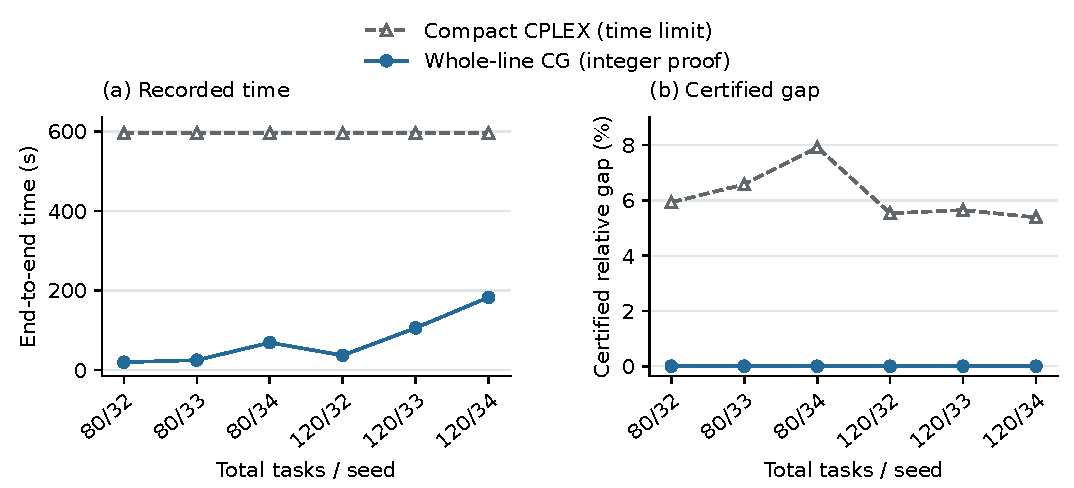
\includegraphics[width=\textwidth]{img/performance_lines.pdf}
\caption{All six paired main inputs, ordered by total tasks and seed: (a) recorded end-to-end time; (b) final certified relative gap. Open triangles indicate time-limited, unproven compact results; filled circles indicate completed decomposition integer proofs. Compact times are censored observations, not times to optimality. Lines connect distinct inputs only as visual guides; they are not convergence trajectories.}\label{fig:runtime}
\end{figure*}
Fig.~\ref{fig:runtime} presents the same comparisons without converting cutoffs into exact speedup ratios. These results support efficient certification on the tested multi-line configurations. They do not establish that the framework first discovers an optimal-profit plan earlier. Comparable first-optimum timestamps are not available for Compact CPLEX.

\subsection{Resource Coordination and a Large-Block Boundary}
\begin{table*}[!t]
\caption{Resource-Constrained and Large-Block Cases Under the 180-Second Protocol}\label{tab:robust}\centering\small
\begin{tabular}{llrrrrrrl}\toprule
Instance $N/L$/seed & $h^{\max}/r^{\max}$ & \multicolumn{3}{c}{Compact CPLEX} & \multicolumn{4}{c}{Whole-line framework}\\\cmidrule(lr){3-5}\cmidrule(lr){6-9}& & LB & UB & Time (s) & LB & UB & Time (s) & Proven\\\midrule
80/2/31 & 6/7 & 693.08 & 733.55 & 175.64 & 569.53 & 738.73 & 174.97 & No\\
120/6/32 & 10/9 & 911.91 & 1010.76 & 175.59 & 927.46 & 927.46 & 30.73 & Yes\\
120/6/33 & 9/10 & 955.90 & 1069.88 & 175.56 & 971.93 & 971.93 & 61.51 & Yes\\
120/6/34 & 10/10 & 980.67 & 1101.05 & 175.55 & 1009.98 & 1009.98 & 144.55 & Yes\\
\bottomrule\end{tabular}
\par\smallskip\begin{minipage}{\textwidth}\footnotesize The 120-task inputs use 80\% of calibrated independent resource use, rounded upward. The 80-task two-line row is the retained large-block boundary. Compact CPLEX is unproven in all four rows.\end{minipage}
\end{table*}

Table~\ref{tab:robust} extends the comparison to stronger resource competition. The framework proves the three 120-task optima under the 180-second protocol. Compact CPLEX remains unproven and returns lower profits. Seeds~32 and~33 close through verified integer plans and complete CG bounds. Seed~34 requires 31 demand-driven profile queries after an incomplete CG pricing round. Its final certificate concerns the original integer optimum. It does not assert complete line-LP convergence.

The two-line case in Table~\ref{tab:robust} provides a contrary result. Two lines with 40 tasks each produce difficult local MILPs. The decomposition returns both a lower profit and a looser UB than Compact CPLEX. Its CG pricing consumes about 156 seconds, and subsequent profile queries do not close the gap. Thus total task count alone does not predict the benefit of decomposition.

The separate 80-task structure study provides further context. A resource-constrained eight-line input reaches the same proven optimum under both methods. The framework completes in about 2.91 seconds; Compact CPLEX completes in about 128.09 seconds. A resource-ample eight-line input instead favors Compact CPLEX, at about 1.24 versus 1.64 seconds. The supplementary tables retain every compact/decomposition pair in that structure study. The evidence supports a tradeoff between block difficulty and coordination, rather than a universal benefit from adding lines.

\subsection{Iterations, Cost, and Interpretation}
\begin{table}[!t]
\caption{Pricing Rounds and Native Solver Costs in the Main Experiment}\label{tab:iterations}\centering\small
\setlength{\tabcolsep}{3pt}
\begin{tabular}{lrrrrrr}\toprule
$N/L$/seed & $i_I$ & $i_{II}$ & PP & Cols. & PP (s) & RMP (s)\\\midrule
80/4/32 & 1 & 3 & 20 & 18 & 17.67 & 0.0064\\
80/4/33 & 1 & 4 & 24 & 22 & 22.79 & 0.0077\\
80/4/34 & 1 & 4 & 24 & 21 & 66.70 & 0.0073\\
120/6/32 & 1 & 3 & 30 & 26 & 34.24 & 0.0058\\
120/6/33 & 1 & 5 & 42 & 28 & 102.94 & 0.0076\\
120/6/34 & 1 & 4 & 36 & 27 & 180.31 & 0.0056\\
\bottomrule\end{tabular}
\par\smallskip\begin{minipage}{\columnwidth}\footnotesize A pricing round includes an RMP solution and at least one pricing attempt under its duals. PP includes economic initialization. RMP-only transition and bound-closure records do not count as pricing rounds. Resource-profile query counts are zero in these six runs.\end{minipage}
\end{table}

Table~\ref{tab:iterations} shows that Phase II needs only three to five pricing rounds in the main experiment. Native pricing nevertheless accounts for about 91--99\% of total framework time. Each RMP uses less than 0.01 second of native solve time. The restricted integer master also remains small. These observations identify local pricing difficulty as the main cost in this regime.

The whole-line formulation can strengthen the relaxation through local integer convexification. It can also simplify integer combination by placing all within-line compatibility inside each column. The experiments are consistent with these mechanisms. They do not isolate relaxation strength from warm-start behavior or solver search-state effects. A full component ablation is still required to quantify each contribution.

The evaluation has a defined boundary. It uses a small synthetic development suite and one solver seed per measured input. Resource calibration is part of the instance construction. The suite does not establish statistical significance, industrial ergonomic validity, or performance on arbitrary large line blocks. Broader comparator algorithms, measured product cases, and an independent final test suite remain necessary before a broad state-of-the-art claim.

\section{Conclusion}\label{sec:conclusion}
This work develops a whole-line decomposition framework for multi-line selective human--robot disassembly with cumulative fatigue. Complete line plans preserve local feasibility and expose only two shared-resource totals to the master problem. Two-phase CG supplies LP coordination and valid bounds. Restricted integer recovery and demand-driven resource profiles supply separate integer witnesses and proof paths.

The tested multi-line configurations show a certification advantage over direct compact-model optimization. The retained large-block case defines a practical limitation: difficult local MILPs can dominate the computation. The results therefore support decomposition for the tested structure, rather than unconditional superiority at larger task counts.

Further investigation concerns stronger line-pricing bounds, allocation of certification budgets, and measured-product validation. Learning-assisted control is a possible extension for candidate generation and certification decisions. The present results contain no trained learning policy or evidence of a reinforcement-learning speedup.

\bibliographystyle{IEEEtran}
\begingroup\fontsize{8}{9.5}\selectfont
\bibliography{MyReferences}
\endgroup
\end{document}
